\section{The Karstaway branch}

 \subsection{Karstaway}

\margininbox{Karstaway}{
     \begin{citemize}
    \item Jack Hare
    \item Tanguy Racine
    \end{citemize}}{\explo}
Zdenko had spoken of an undescended pitch just waiting to be dropped at the end of \passage{Galerija}. I'd not yet been as deep into \passage{Primadona} as that, and with few others looking to cave, Tanguy and I had a chance to go check out this juicy lead.
 
\begin{marginfigure}
\checkoddpage \ifoddpage \forcerectofloat \else \forceversofloat \fi
\centering
 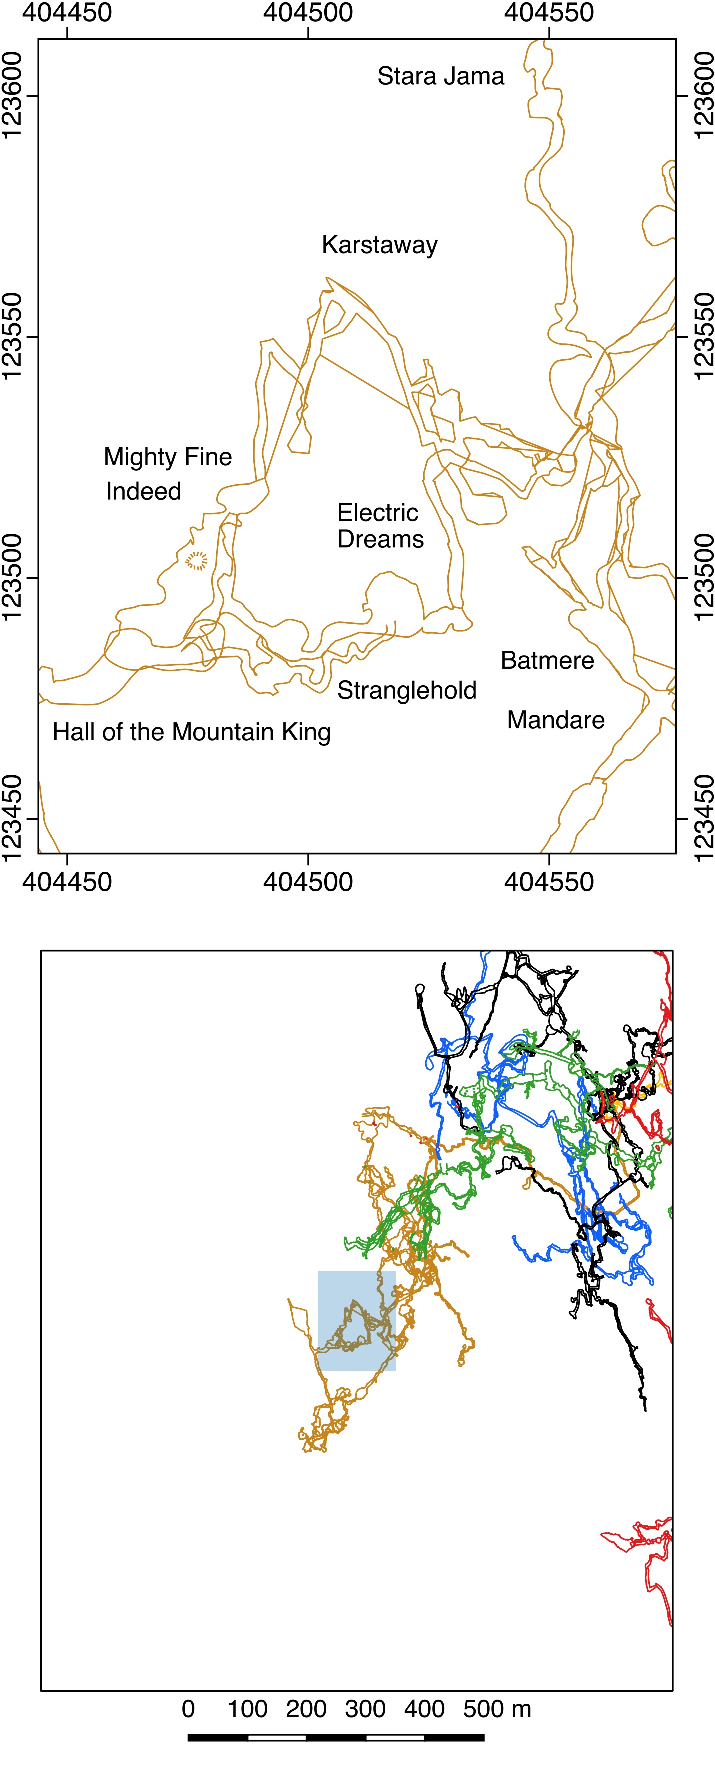
\includegraphics[width=\linewidth]{images/little_insets/hotmk_inset.pdf}
 \caption{Plan view of the \protect\passage{Tight and Scrotty} extensions over the top of the \protect\passage{Upside Down Chamber} chamber. Slovenian National Grid ESPG 3794}
 \label{karstaway inset}
\end{marginfigure}

I had the chance to do \passage{Risanke} for the first time, and found the squeeze very tight and unpleasant. The pitches had been rebolted closely following the Slovenian's expedition rigging, which was less than ideal and some of them were rebolted over the rest of the expedition. We were unclear on many of the Slovenian names for parts of the system, and several were anglicised, so \passage{Sejna Soba} (the drawing room) became \passage{Sane and Sober}, two things the \passage{Migovec} cavers cannot fairly be accused of being. Given this, we soon arrived at \passage{Knot Very Good}, at the bottom of which \passage{Smer0} and \passage{Galerija} head off.
 
We passed over some big holes in the ground of \passage{Galerija}, the slick mud always slightly unnerving, and free climbed over the top of \passage{Quantum State}, which had been dropped the previous day. Afterwards, this traverse was bolted, but we lacked a drill and rope and made up for it with bravado and a sense of our own invincibility.
 
The passage on the other side is a hading rift which develops into a fossil streamway. One steep downclimb caused me to remark that we'd have difficulty with it on the way back up, which Tanguy later took as a challenge. At the end of the passage we found a howling draft and a yellow tackle sack, abandoned by the JSPDT years ago. The pitch was not undescended -  a rope of unknown provenance lead off and round a buttress on the right.
 
Tanguy did the only sensible thing and let me go first. Lowering myself onto the old rope I edged out round the corner to see a massive drop beneath me. The shaft is around 15\,m wide, clean washed and fluted walls and 30\,m deep. The pitch is rigged as a single hang of a single dodgy home made hanger (later backed up with a through bolt to form the world's most adorable little Y-hang, but that was later). I descended slowly, not really at ease, and at the bottom took a long, relaxing piss in the one hole I had determined wasn't a lead.
 
There were a few ways off to check out, but Tanguy and I were in full glory hound mode and we focused on the wide fossil streamway. A few free climbs later and the drops were getting bigger. Eventually we got to a big chamber with a ledge on the left wall and a 5\,m drop. Not wanting to give up, I edge along the ledge until the chamber closed back into a rift and I could down climb using ledges on either side. Tanguy followed, not exactly convinced we'd ever get out, and we got to the \passage{Lunch Spot}, my favourite little chamber. Upstream was a flat floored aven with water coming in, and downstream was pristine dark mud. But first, mackerel.
 
 
 \begin{figure*}[t!]
\checkoddpage \ifoddpage \forcerectofloat \else \forceversofloat \fi
\centering
\frame{\includegraphics[width=\textwidth]{"images/2016/jack-middle-2016/jackbolting".jpg}}
\caption{Jack hammers the M8, stainless steel raul bolt we use on expedition to secure a traverse line over \protect\passage{Mighty Fine Indeed} 3rd Pitch, a respectable P42, before drilling in a signature Y-hang: an airy take-off over a diminishing ledge which provides a beautifully clean hang \pic{Tanguy Racine}}
\label{bolt M8}
\end{figure*}

Suitable re-energised we pushed downstream, immediately encountering a nasty squeeze that you had to climb up into. A wet aven followed where we set up a bottle to catch water, and then we followed the water, traversing over the top (a later attempt to follow the water proved tight and unpleasant). Alternating between boulder scrambles and muddy floored chambers, we felt a mounting sense of excitement as the draft kept luring us onwards.
 
Twice we went down through the rift. The first time lead to a narrow chamber with a 10\,m drop that I foolishly decided I could climb out over in search of another way down. Just as Tanguy told me this was a bad idea, my hand hold broke off and I beat a hasty retreat. This is a lead -- we never went back, and there's an undescended pitch just waiting \sidenote{This passage was pushed to its too-tight termination in 2017 and named \protect\passage{Entirely My Fault}}.
 
The other route down was in a hading rift that we slowly squeeze down through until we got sketched out by how far it went. It could use some ropes and another good looking at. The proper route went along at the highest level, and eventually terminated in a 20\,m pitch\sidenote{This formed the other part of \protect\passage{Entirely My Fault}}.
 
On the way back we enjoyed the terrifying free climb back onto the ledge (never again attempted, it was bolted the next day as an unpleasant short pitch) and then up the long rope in \passage{Karstaway}, hoping that the old bolt held. Tanguy built an incredible cairn in a fit of madness in order to pass one free climb, and we surveyed out to an old Slovene PSS that Rhys and Will pointed out to us. We returned to the surface with tales of an incredible lead waiting deep in the mountain.

\subsection{Mighty Fine Indeed}
\margininbox{Mighty Fine Indeed}{
\begin{citemize}
    \item Jack Hare
    \item Rhys Tyers
    \end{citemize}}{\explo}
    
It was easy to lure Rhys on a pushing trip the next day, as I promised increasingly deep and impressive shafts. Equipped with a drill, some scavenged rope and plenty of fish, we ambled down the increasingly familiar series of pitches, pausing to rebolt or re-rig some ropes. At the top of the 30\,m \passage{Karstaway} pitch, we added a second bolt to make a tiny Y-hang and back up the terrifying home-made hanger. Satisfied it was now safe, we continued down, bolting the dodgy free climb down to the \passage{Lunch Spot} chamber to make it a very awkward short pitch.
 
We were both quite excited to make it to the end of \passage{Karstaway}, and looked down at the chamber below. Rhys quickly bolted a back up and a Y-hang, and we descended into a circular chamber with a rift cutting through on the far side. \bignote{Above the rift were huge, flake shaped boulders that seemed improbably perched}, and I avoided thinking about what propped them up. Rhys was already bolting the next section, a sort of steeply descending traverse using the dodgy old rope we were recycling from further up the cave. He dropped down and declared we were out of rope, but by descending onto a ledge and then free climbing down we made it to a flat section in the rift.
 
From here, the passage continued on, but without a floor. Chucked rocks and loud whoops confirmed something huge and impressive lurked just around the corner, but we were out of rope and almost out of time, having spent much of the rest of the day rebolting. The only thing left to do was to name these two pitches. We \emph{ummed} and \emph{arred} until we recalled the words of `Captain Kangaroo', and reinterpreted them as an instruction: `A parallel shaft series would be \passage{Mighty Fine Indeed}.'

\subsection{Hall of the Mountain King}
\margininbox{\footnotesize{Hall of the Mountain King}}{
     \begin{citemize}
    \item Jack Hare
    \item Will Scott
    \item Tanguy Racine
    \item Andrej Fratnik
    \end{citemize}}{\explo}
    
Rhys and I had left the previous day with an undescended pitch into a massive cavern waiting at the bottom of \passage{Mighty Fine Indeed}. It took no effort at all to lure Will Scott back underground, and Tanguy was keen to see where \passage{Karstaway} led. Even better, we were joined by the legendary Andrej Fratnik, who I'd not caved with before. I'd spotted him hiding behind a tree in the woods a few days before, and he greeted me with `you're the one who hunted me'.
 
At the bottom of \passage{Mighty Fine Indeed} the others patiently waited as I bolted a few backups and then nervously edged out over the void. The bottom had eroded out of the old streamway, leaving thin ledges on either side wide enough to stand on. I was determined to get as far along this rift as possible to get a nice clean drop, and soon I was around the corner, out of sight from the others.  
 
The passage widened, and I realised this was the time to descend. The experience Kenneth and I gained rebolting the Super Highway a few days earlier came in handy as I identified a good place for a nice wide Y-hang, one bolt on either wall and the knot hanging at waist height. With hundreds of metres of rope attached to my side I felt pretty confident about reaching the bottom, but I still paused for a while checking and rechecking every bolt, knot and maillon. Finally there was no further excuse to linger, and I began to descend.
 
My light was not bright enough to see anything but the closest wall. The darkness below me was absolute, and soon \bignote{all I could see above me were the faint lights of my friends}. Some way down the wall began to get closer, and I realised the rope would soon rub. I panicked slightly, never having put in a rebelay before, but calmed myself as I dangled twenty or so metres below the last anchor and hard locked my descender, swinging to the left and wedging a leg into a rift. My first bolt was badly placed, causing the knot to rub, but I think I didn't correct it, leaving the flaw for Tanguy to identify. 
 
Descending again and I began to get wet, some drops seeping through a bedding plane and forming a little waterfall. I could see the shaft continued down for another ten metres, but most of the chamber was higher up, and there was a little ledge around which I could traverse and step off into the chamber. A few bolts later and I was done, and I called for the others to join me.
 
I sat in the vast chamber (later called `\passage{Hall of the Mountain King}', as Andrej joined in as I hummed it), my light off, mentally exhausted by the descent, as my friends joined one by one, splitting up and scouring the chamber for the next lead. I felt entirely spent, but overjoyed - \bignote{here was the exploration of vast, unknown chambers which I had promised myself}. Soon my strength returned and I went to see what we had found.
 
The chamber formed inside a huge sinuous rift, with the ceiling far above and the floor strewn with massive boulders. I followed the sound of voices around a corner, and found the floor rose up, a scramble over boulders that terminated in a wall at the end. Here I saw Tanguy, who had, against all sanity and the laws of physics, scrambled up a dangerous, unprotected rock face and was now stranded five metres off the ground. He implored us to pass him up a rope and a drill, with which he proceeded to rig by far the worst pitch I've ever seen. It rubbed, it swung, the rebelay was too tight, the pitch head unprotected and there were numerous loose rocks and boulders peering excitedly over the rim onto us below.

There was nothing for it but to join the crazed Frenchman. \bignote{Will was unsure, Andrej was stoic and I was resigned} as we climbed, cursed and swung, making it to a small saddle at the top of the wall which lead to a down-climb on the other side. It appeared to a long gallery, which ran NW to SE, and we had intercepted it half way along. The draft here was impressive, so we decided to follow it, picking our way along a nice wide passage.
 
Half way along we encountered a short free climb down, but it was just high enough to be intimidating. Tanguy tried to force himself into a rift in the side wall, reckoning this was the way down, but became wedged. I wriggled through a rift in the floor, and as I popped through I heard the sounds of an animal in severe distress. I enquired whether everything was okay, but all I got was Tanguy imploring everyone to stand clear. The pressure on his bowels being too much, Tanguy wrenched himself from the rift and deposited a massive, steaming turd in the centre of our newly discovered passage directly upstream of the lead. The new passage was named `\passage{Colony}', as it was a bit.
 
I was trapped on the other side from my comrades, who had retreated with some speed back the way we had come. As Tanguy cleaned himself up as best he could, I looked around to assess the situation. At a lower level there seemed to be a passage back the way we had come, and I followed it up, popping out where we had stopped for lunch. I hailed the others, who were grateful for an alternative route, and \bignote{we soon regrouped on the far side of Tanguy's shit}.

\begin{pagefigure}
    \centering
    \begin{subfigure}[t]{0.393\textwidth}
        \centering
        \frame{\includegraphics[width=\linewidth]{"images/2016/jack-middle-2016/hall_of_the_mountain_king2".jpg}} 
        \caption{(a)} \label{Hall of the Mountain King}
    \end{subfigure}
    \hfill
    \begin{subfigure}[t]{0.59\textwidth}
        \centering
        \frame{\includegraphics[width=\linewidth]{"images/2016/jack-middle-2016/surveying_colony".jpg}} 
        \caption{(b)} \label{Colony}
    \end{subfigure}

    \vspace{0.3cm}
    \begin{subfigure}[t]{\textwidth}
    \centering
        \frame{\includegraphics[width=\linewidth]{"images/2016/jack-middle-2016/bottom_of_blue_danube".jpg}} 
        \caption{(c)} \label{Bottom of Blue Danube}
    \end{subfigure}
    
    \caption{
    \textit{(a)} Jack Hare, Will Scott and Andrej Fratnik surveying the 42\,m drop into \protect\passage{Hall of the Mountain King} chamber
    \textit{(b)} Will Scott surveying the climb into \protect\passage{Colony}
    \textit{(c)} Jack Hare and Will Scott starting the survey at the bottom of \protect\passage{Blue Danube}, P46 \pic{Tanguy Racine}}

\end{pagefigure}


The draft was enticing and the stench was powerful [Ed: Okay, that's enough now] as we continued down the passage. Soon we encountered another huge shaft, with a chamber coming off to the side. To have one such find in a day was remarkable - to have two began to look greedy. Tanguy was itching to get down, and I casually mentioned that he'd just `waltz down it', leading to it being named \passage{Blue Danube}.

As Will and Andrej surveyed back to our lunch spot, I scrambled in the SE direction into unexplored passage to see if it died quickly. It didn't - instead, there were a few free climbs as the hading rift filled with boulders, and there was a thick brown mud on the floor. After a hundred metres of this I realised I was being greedy, and I built a cairn and turned round, willing this lead to another group (I was soon back with Kenneth to christen it `\passage{What a Coincidence}'.)
 
We returned to find Tanguy descending from a hanging rebelay, and we followed down. The top was a bit loose as Tanguy was slightly too keen to garden properly, and half way down \bignote{there was a ledge far away on the other side, leading to a vast chamber} which Rhys and Arun would explore as \passage{Upside Down Chamber}.\sidenote{Interestingly, this ``shaft next to a big chamber'' setup is very similar to \passage{Galaktika}.}
 
Instead, the rope dropped down a clean washed shaft, ten metres in diameter with beautiful grey scalloped walls. At the bottom, the water pooled and ran off into a tight rift that immediately became a pitch. It had been a long day and there was much to survey, so we turned round. Andrej's approach to accuracy consisted of waving the laser disto near the next station and shouting numbers rounded to the nearest ten metres, but with this approach we made rapid progress, singing Simon and Garfunkel as we crept back through the \passage{Hall of the Mountain King}. Tanguy's shit stained upper passage was never surveyed, and the survey contains only an artist's impression of the best decorated cave passage in Slovenia.

\name{Jack Hare}


